%% Libs
\documentclass[polish,11pt,a4paper]{article}
\usepackage[a4paper, margin=1.5cm]{geometry}
\usepackage[T1]{fontenc}
\usepackage{babel}
\usepackage{graphicx}
\usepackage{ragged2e}
\usepackage{caption}
\usepackage{amsmath} 
\usepackage{amssymb} 
\usepackage{setspace}
\usepackage[utf8]{inputenc}
\usepackage{subfig}
\usepackage{cancel}
\usepackage{import}
\usepackage{svg}
\usepackage{pdfpages}
\usepackage{geometry}
\usepackage{multicol}
\usepackage{float}
%% start document
\begin{document}
	%% Strona tytułowa
	\setstretch{1}
	\centering
	\section*{WYDZIAŁ MECHANICZNY POLITECHNIKI BIAŁOSTOCKIEJ}
	\begin{figure}
		\centering
		\includegraphics[width=0.4\linewidth]{logo}
		\label{fig:logo}
	\end{figure}
	
	\section*{PROJEKT Z PRZEDMIOTU}
	\section*{Systemy Autonomiczne}
	\large
	kod przedmiotu: MYAR2S22007M
	\subsection*{Temat: Projektowanie układu sterowania i nawigacji
		śmigłowca wielowirnikowego jako systemu
		autonomicznego }
	\vspace{1cm}
	\raggedright
	Autor: Ostaszewicz Dawid
	
	Kierunek: Automatyka i Robotyka, II stopień
	
	Specjalność: Informatyzacja Przemysłu
	
	Semestr II
	
	Prowadzący: dr inż. Leszek Ambroziak
	\vspace{1cm}
	
	Weryfikacja efektów uczenia się:
	
	EK1: \dotso
	
	EK2: \dotso
	
	EK3: \dotso
	
	EK4: \dotso
	
	EK5: \dotso
	
	EK6: \dotso
	
	EK7: \dotso
	
	EK8: \dotso
	
	Uwagi prowadzącego:
	\vspace{2cm}
	
	ocena: \dotso
	\clearpage
	
	% Koniec strony tytulowej
 	\multicols{2}
 	\justifying
\section*{Cel i zakres projektu}

Celem projektu jest zgłębienie zagadnień związanych z systemami autonomicznymi na przykładzie śmigłowca wielowirnikowego. Zakres prac obejmuje analizę modelu śmigłowca, mechanizmów autonomii lotu oraz algorytmów umożliwiających skuteczne planowanie trajektorii, generowanie linii drogi i jej aktywną korekcję. 


\section*{Opis modelu}
Śmigłowiec czterowirnikowy, określany również jako quadrotor lub quadkopter, to bezzałogowy statek powietrzny zdolny do pionowego startu i lądowania (ang. VTOL – vertical take-off and landing). Wyposażony jest w cztery śmigła generujące siłę nośną (ang. lift force), napędzane przez silniki, które pracują w parach, obracając się w przeciwnych kierunkach (dwa zgodnie z ruchem wskazówek zegara, a dwa przeciwnie). Schemat ogólny konstrukcji przedstawiono na rys. \ref{fig:model}. Sterowanie śmigłowcem odbywa się poprzez regulację prędkości obrotowej poszczególnych śmigieł. Ruch w osi pionowej z realizowany jest realizowany jest przez jednoczesną zmianę prędkości wszystkich czterech śmigieł. Przemieszczenie w osi x uzyskuje się, modyfikując prędkości wirników 1 i 3, pozostawiając prędkości wirników 2 i 4 niezmienione. Analogicznie, ruch wzdłuż y osi  można osiągnąć, zmieniając prędkości wirników 2 i 4, przy zachowaniu stałej prędkości wirników 1 i 3.

\begin{figure}[H]
	\centering
	\includegraphics[width=0.7\linewidth]{model}
	\caption{Schemat śmigłowca czterowirnikowego}
	\label{fig:model}
\end{figure}

Siła ciągu generowana przez każdy element napędowy może zostać określona (\ref{eq:ciag})

\begin{equation}
	T_i = b \omega_i^2 \quad gdzie \, \, i = 1,2,3,4
	\label{eq:ciag}
\end{equation}
\textit{b} to współczynnik siły nośnej zależny od gęstości powietrza, skoku śmigieł, średnicy oraz liczby łopat. W układzie globalnym {A} stosując drugą zasadę dynamiki Newtona możemy zapisać następujące równanie dla ruchu translacyjnego śmigłowca (\ref{eq:ruch})
\begin{equation}
	m\dot{v} = 
	\left(
		\begin{matrix}
		0 \\
		0 \\
		mg \\
		\end{matrix}
	\right) - ^{A}R_{B}
		\left(
	\begin{matrix}
		0 \\
		0 \\
		T \\
	\end{matrix} \right)
	\label{eq:ruch}
\end{equation}
\textit{v} jest prędkością w układzie związanym z Ziemią, \textit{g} to stała grawitacyna, \textit{m} jest masą śmigłowca, natomiast \textit{T} jest sumarycznym ciągiem zdefiniowanym (\ref{eq:sum}) 
\begin{equation}
	T = \sum T_i
	\label{eq:sum}
\end{equation}
Różnice w prędkości obrotowej śmigieł powodują powstanie momentu, co możemy zapisać dla obrotu wokół osi x. Jeśli \textit{d} jest długością ramienia, wtedy uwzględniając zależności (\ref{eq:ciag}); wartości momentów w osi \textit{x} i \textit{y} można zapisać następująco (\ref{eq:tx}, \ref{eq:ty})
\begin{equation}
	\tau_x = db(\omega_4^2 - \omega_2^2)
	\label{eq:tx}
\end{equation}
\begin{equation}
	\tau_x = db(\omega_3^2 - \omega_1^2)
	\label{eq:ty}
\end{equation}
Na każde śmigło działa siła oporu aerodynamicznego, która może być zdefiniowana jako (\ref{eq:opor})
\begin{equation}
	\mathcal{Q}_i = k \omega_i^2
	\label{eq:opor}
\end{equation}
\textit{k} tak samo jak \textit{b} zależy od czynników takich jak gęstość powietrza, skoku śmigieł, średnicy czy liczby łopat  i jest współczynnikiem oporu aerodynamicznego. Moment wokół osi z jest zdefiniowany (\ref{eq:mz}).
\begin{equation}
	\tau_z = \mathcal{Q}_1 - \mathcal{Q}_2 + \mathcal{Q}_3 - \mathcal{Q}_4 = k(\omega_1^2 - \omega_2^2 + \omega_3^2 - \omega_4^2) 
	\label{eq:mz}
\end{equation}
Ruch obrotowy śmigłowca jest opisany równaniem (\ref{eq:in}).
\begin{equation}
	\mathbf{J}\dot{\omega} = -\omega \times \mathbf{J}\omega + \Gamma
	\label{eq:in}
\end{equation}
Siły i momenty (\ref{eq:out}) są funkcjami prędkości obrotowych śmigieł.
\begin{equation}
	\begin{pmatrix}
		T \\ 
		\mathbf{\Gamma}
	\end{pmatrix} = 
	\begin{pmatrix}
		-b & -b & -b & -b \\ 
		0 & -db & 0 & db \\ 
		db & 0 & -db & 0 \\ 
		k & -k & k & -k
	\end{pmatrix}
	\begin{pmatrix}
		\omega_1^2 \\ 
		\omega_2^2 \\ 
		\omega_3^2 \\ 
		\omega_4^2
	\end{pmatrix}
	\label{eq:out}
\end{equation}
W przedstawionej sytuacji wektor stanu jest następujący (\ref{eq:stan}).
\begin{equation}
	\mathbf{x} = (x, y, z, \phi, \theta, \psi, \dot{x}, \dot{y}, \dot{z}, \dot{\phi}, \dot{\theta}, \dot{\psi})^T
	\label{eq:stan}
\end{equation}
\textit{$x$,$y$,$z$} to parametry określające położenie śmigłowca w przestrzeni trójwymiarowej \textit{$\phi$, $\theta$, $\psi$} oznaczają kolejno kąt przechylenia, pochylenia i odchylenia, następnie wektor zawiera ich pochodne. Model opisany w ten sposób jest dostępny w bibliotece Robotics and Machine Vision Toolbox. Według dokumentacji Peter'a Corke'a, wstawienie własnych parametrów modelu odbywa się w pliku \textit{mdl\_quadrotor.m}. Do poprawnego wykonania ćwiczenia trzeba ustawić własne parametry modelu. W tym wypadku należą do grupy 10; $M$ = 5.89, $I_{xx}$ = $I_{yy}$ 0.1003, $I_{zz}$ = 0.1619, $d$ = 0.364.
\section*{Zadanie 1}
\subsection*{Treść}
Celem tego zadania jest zapoznanie się z układem symulacyjnym śmigłowca czterowirnikowego dostępnym w bibliotece RMVT. Należy wprowadzić modyfikacje, które umożliwią wyświetlanie parametrów lotu śmigłowca, porównując wartości zadane parametrów nawigacyjnych z aktualnie mierzonymi. Kolejnym krokiem jest dostosowanie modelu dynamiki śmigłowca do parametrów zawartych w tabeli, a następnie sprawdzenie działania układu sterowania z nowymi wartościami. Należy przeanalizować wpływ zmian na stabilność modelu, dostosowując nastawy pętli regulacyjnych i metody stabilizacji śmigłowca. Dodatkowo, warto przeprowadzić eksperymenty z różnymi wartościami wzmocnienia w układzie sterowania, szczególnie badając efekty zmniejszenia tłumienia lub jego całkowitego usunięcia. Można również usunąć kompensator siły grawitacji i sprawdzić, jak zmienia się działanie układu przy dużym wzmocnieniu w układzie sterowania wysokością lub zastosowaniu alternatywnego regulatora.
\subsection*{Opracowanie}
Dynamika śmigłowca jest silnie uzależniona od jego masy oraz właściwości tensora bezwładności. W celu rozpoczęcia strojenia regulatorów, na wejścia obiektów zostały zastosowane sygnały skoku jednostkowego, co pozwoliło na ocenę odpowiedzi układu na zmiany parametrów. Układ regulacji składa się z kaskadowo połączonych pętli, a strojenie powinno zaczynać się od najbardziej wewnętrznych pętli, czyli od regulatorów odpowiedzialnych za kontrolę postawy ("attitude control"). W systemie regulacji wyróżnia się pętle regulacji: położenia, prędkości i wysokości, z czego prędkość zależy od kątów położenia śmigłowca. Regulacja położenia śmigłowca odbywa się poprzez kontrolę kątów roll i pitch, które wpływają na zadane prędkości.

Zgodnie z tym podejściem, proces strojenia rozpoczęto od regulatorów znajdujących się w najbardziej zagnieżdżonych pętlach, stopniowo przechodząc do obszarów nadrzędnych w układzie regulacji. Efektem strojenia powinna być trajektoria całkowicie aperiodyczna, ponieważ jakiekolwiek przeregulowanie może stanowić zagrożenie dla bezpieczeństwa śmigłowca. Odpowiedzi uzyskane w wyniku strojenia zostały zaprezentowane na Rysunkach \ref{fig:xyz} i \ref{fig:RLY}.


\begin{figure}[H]
	\centering
	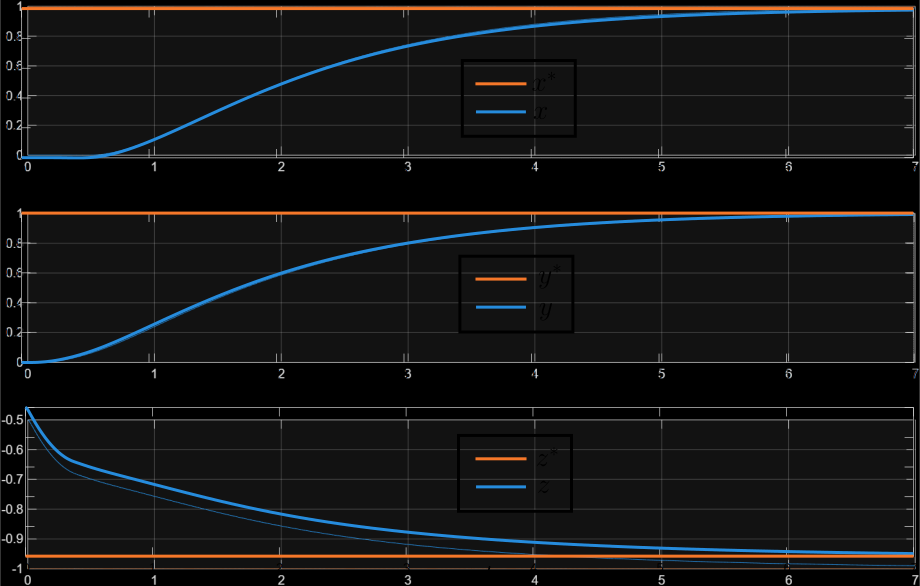
\includegraphics[width=1\linewidth]{strojenie/XYZ}
	\caption{Odpowiedź skokowa - xyz}
	\label{fig:xyz}
\end{figure}

\begin{figure}[H]
	\centering
	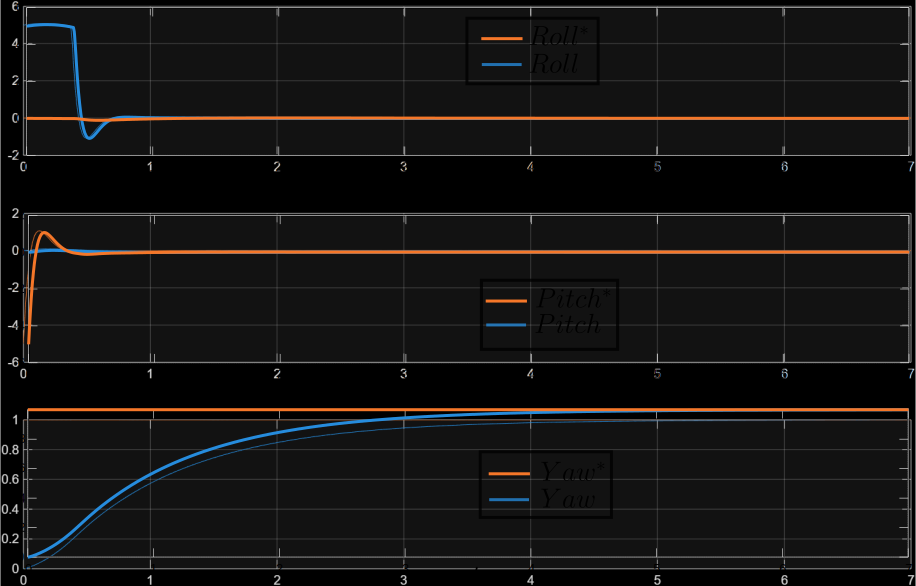
\includegraphics[width=1\linewidth]{strojenie/RLY}
	\caption{Odpowiedź skokowa - RLY}
	\label{fig:RLY}
\end{figure}

Do układu regulacji wysokości kluczowe było odpowiednie ustawienie zmiennej "thrust feedforward", ponieważ 
układ powienien odpowiednio kompensować wpływ grawitacji. Nastawy regulatorów zostały zestawione w Tabeli 1.

\begin{figure}[H]
	\centering
	\includegraphics[width=1\linewidth]{nastawy}
\end{figure}
Jeśli chodzi o zmienną "thrust feedforward", można odpowiednio nastroić regulator wysokości bez niej, jednak wiąże się to z
efektami, które mogą nie być wygodne, lub możliwe do realizacji. Rysunek 4, przedstawia dziłanie nastaw dla regulatora
wysokości z zerową nastawą "Thrust feedforward" z tabeli 1.

\begin{figure}[H]
	\centering
	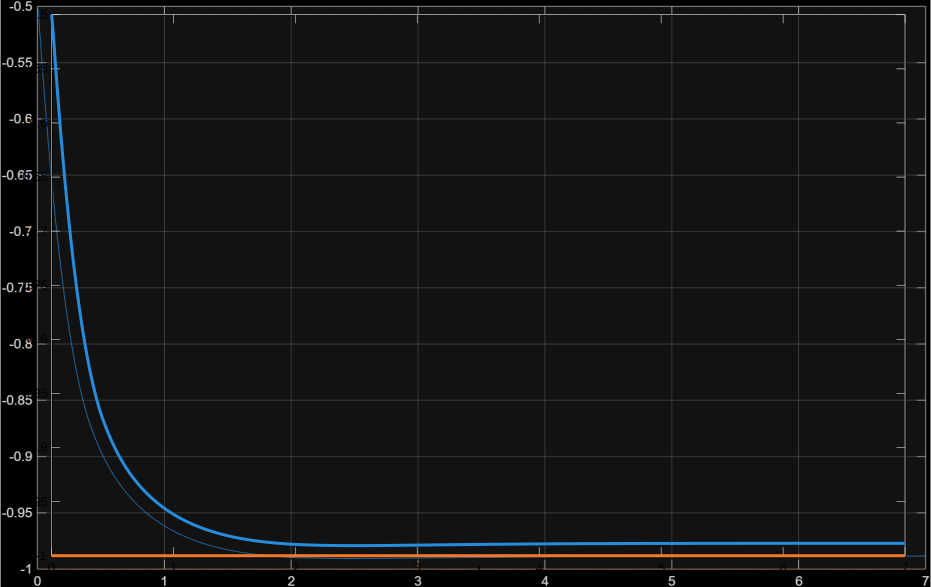
\includegraphics[width=1\linewidth]{strojenie/z.png}
	\caption{Odpowiedź układu dla strojenia bez kompensatora grawitacji}
	\label{fig:sz}
\end{figure}

Trzeba zauważyć, że przy takim strojeniu wielkości w torze sygnałów sterowania będą miały bardzo duże wartości
na wyjściach regulatorów, co w większości przypadków może nie być możliwe w realizacji. Poza tym układ posiada jeszcze
mały uchyb.

\subsection*{Podsumowanie}
Strojenie regulatorów powinno zaczynać się od wewnętrznych pętli regulacji, a następnie przechodzić do pętli nadrzędnych. W przypadku regulatora wysokości, jego strojenie można przeprowadzić bez zastosowania kompensatora wysokości, jednak w praktycznej realizacji takie podejście może prowadzić do trudności w utrzymaniu stabilności lub wymagania większej precyzji w kontrolowaniu ruchu. Kompensator wysokości pomaga w eliminacji błędów i poprawia jakość działania regulatora w warunkach zmiennych obciążeń lub zakłóceń.

\section*{Zadanie nr 2}
\subsection*{Treść}
Opracuj funkcję realizującą ruch balistyczny śmigłowca. Niech quadrotor wystartuje
pod kątem 45 stopni do poziomu, następnie wyzeruj cały ciąg. Sprawdź uzyskaną trajektorię śmigłowca.
Spróbuj opracować funkcję realizującą lot balistyczny do zadanego punktu na powierzchni.

\subsection*{Opracowanie}
Istnieje kilka metod realizacji ruchu balistycznego śmigłowca wielowirnikowego. Jednym z podejść jest sterowanie śmigłowcem w kierunku określonego punktu w przestrzeni, a następnie, w trakcie przyspieszania, wyłączenie lub ograniczenie ciągu. Dzięki temu trajektoria lotu powinna zbliżyć się do trajektorii balistycznej. W praktyce, jednak, to rozwiązanie może napotkać trudności związane z precyzyjnym uchwyceniem momentu, w którym ciąg powinien zostać wyłączony, ponieważ zbyt późne wyłączenie może skutkować niewystarczającym przyspieszeniem w osiach XY, co utrudnia uzyskanie prawidłowej trajektorii balistycznej. Prostszym podejściem może być ustawienie pozycji śmigłowca, która będzie rosła liniowo w czasie. W przypadku zastosowania regulatorów o pojedynczym całkowaniu, śmigłowiec nie będzie w stanie precyzyjnie nadążyć za wartością zadaną, co skutkuje stałym uchybem. Niemniej jednak, obiekt w tej metodzie utrzyma stałe przyspieszenie, a po ograniczeniu ciągu zacznie się zniżać, co pozwoli uzyskać trajektorię zbliżoną do balistycznej. 
Ciąg generowany przez śmigła będzie ograniczany, w różnych odstępach czasu. Badanie odległości punktu
lądowania od czasów wyłączenia, umożliwi wyprowadzenie zależności czasu ograniczenia ciągu od odległości;
ostatecznie taki zabieg umożliwi stworzenie relacji, która pozwoli zadawać punkt lądowania.
Znając relację czasu wyłączenia od odległości na jakiej ląduje dron (można obliczyć z eq 11).
\begin{equation}
	s = \sqrt{x^{2}+y^{2}}
\end{equation}
Można z pomocą Rysunku 7 aproksymować odległość punktu lądowania. W takim kontekście zadanie punktu lądowania powinno odpowiadać
wektorowi przemieszczenia w płaszczyźnie XY i relacji czasu ograniczenia ciągu. Pierwszą rzeczą będzie zadanie określenia kąta wektora przemieszczenia
w płaszczyźnie XY, eq (12, 13)


\begin{equation}
	k_{x} = \sin \arctan \frac{x^{*}}{y^{*}}
\end{equation}

\begin{equation}
	k_{y} = \cos \arctan \frac{x^{*}}{y^{*}}
\end{equation}
Natomiast moduł wektora przemieszczenia określa równanie aproksymacji drogi eq (14)

\begin{equation}
	t = \sqrt{x^{2}+y^{2}} - 0.13
\end{equation}

\begin{figure}[H]
	\centering
	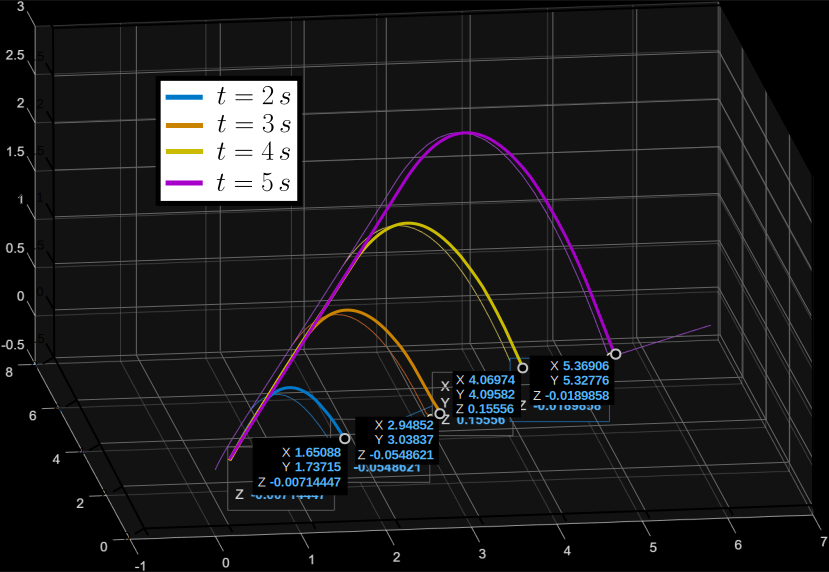
\includegraphics[width=\linewidth]{paraboliczna/parabole.png}
	\caption{Otrzymane trajektorie balistyczne}
\end{figure}

\begin{figure}[H]
	\centering
	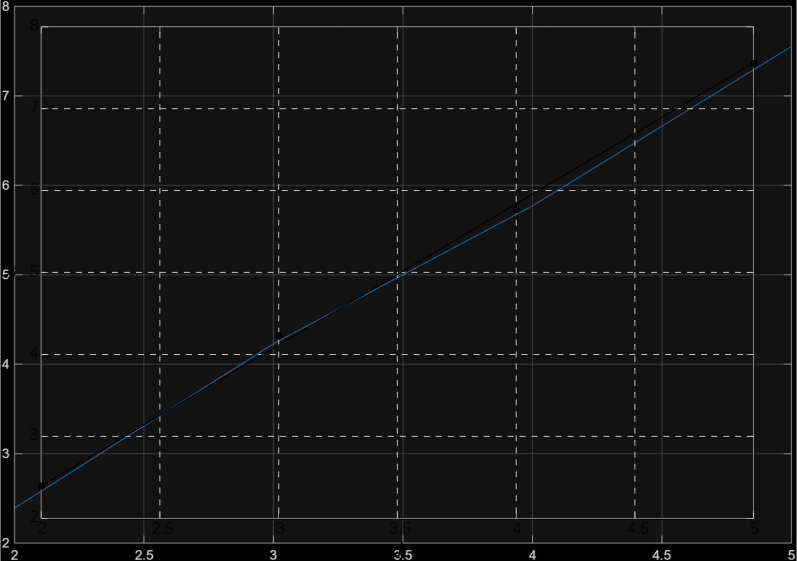
\includegraphics[width=\linewidth]{paraboliczna/st.png}
	\caption{Odległość od punktu startowego}
\end{figure}

\subsection*{Wnioski}
Wykonane badania pozwoliły na określenie zależności niezbędnych do realizacji balistycznego lotu śmigłowca wielowirnikowego. Zastosowanie liniowo narastających wartości zadanych umożliwia ustalenie stałego przyspieszenia obiektu, podczas gdy ograniczenie ciągu wymusza ruch po trajektorii balistycznej. Przeprowadzone badanie, wraz z odpowiednią aproksymacją, pozwala na wyprowadzenie równań opisujących lot balistyczny w przybliżeniu do punktu zadanego.

\section*{Zadanie nr 3}
\subsection*{Treść}
Opracuj funkcję realizującą automatyczne lądowanie śmigłowca w oparciu o dostępne 
sygnały pomiarowe (lądowanie może być aktywowane w dowolnym momencie, ze wskazaniem miejsca laowania,
po aktywowaniu funkcji automatycznego lądowania śmigłowiec przerywa wcześniej realizowany scenariusz,
podąża do punktu lądowania, przechodzi do zawisu, po czym łagodnie ląduje)
\subsection*{Opracowanie}
Pierwszą fazą lądowania jest przerwanie czynności, które obecnie są realizowane przez drona. Wartości
zadane w osiach x i y będą zapamiętywane przy użyciu bloku z Rysunku \ref{fig:mem}

\begin{figure}[H]
	\centering
	\includegraphics[width=1\linewidth]{lądowanie/set.png}
	\caption{Funkcja pamięci stanu trajektorii w płaszczyźnie xy}
	\label{fig:mem}
	
\end{figure}

Funkcja zapamiętuje wartości, które dron następnie utrzymuje. W tej fazie lądowania dochodzi również do zniżania pułapu lotu do wartości około 30 cm przy użyciu przełącznika. Założenie drugiej fazy lądowania zakłada, że jeśli dron osiągnie pułap mniejszy niż 35 cm, rozpocznie stopniowe ograniczanie ciągu silników. W trzeciej fazie, po osiągnięciu pułapu 20 cm, silniki zostaną wyłączone, aby zminimalizować turbulencje związane z oddziaływaniem z podłożem. Wnętrze bloku automatycznego lądowania przedstawia Rysunek \ref{fig:lond}.
\begin{figure}[H]
	\centering
	\includegraphics[width=\linewidth]{lądowanie/lond.png}
	\caption{Automatyczne lądowanie - blok}
	\label{fig:lond}
	
\end{figure}

Wejście set jest związane z działaniem przycisku. W trakcie lotu można przełączyć przełącznik, który rozpocznie
sekwencję automatycznego lądowania. Wnętrze bloku matlab function:
\begin{footnotesize}
	\begin{verbatim}
		function w = fcn(sw,z)
		
		if (z > -0.35) && (z < -0.30)
		w = 0.8*sw;
		elseif (z >= -0.30) && (z < -0.20)
		w = 0.6*sw;
		elseif (z >= -0.20)
		w = 0.1*sw;
		else
		w = sw;
		end
	\end{verbatim}
\end{footnotesize}
\begin{figure}[H]
	\centering
	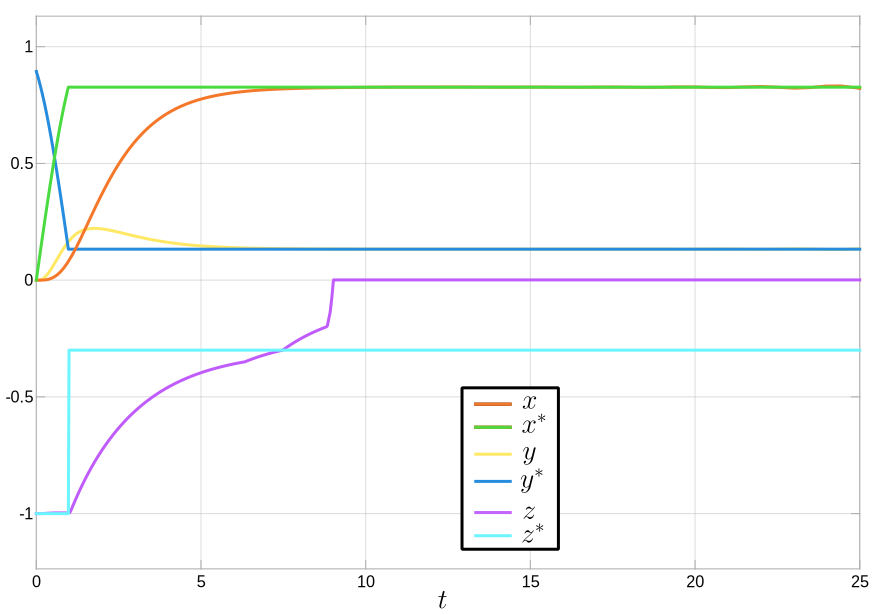
\includegraphics[width=\linewidth]{lądowanie/land.png}
	\caption{Automatyczne lądowanie - sygnały}
\end{figure}
\subsection*{Podsumowanie}
Po czasie około sekundy przełącznik automatycznego lądowania został włączony, zmienił wartość wejścia "set" bloku automatycznego
lądowania. Następnie zadane trajektorie zostały wstrzymane na jednym punkcie w płaszczyźnie xy; następowało 
zniżenie pułapu lotu, następnie układ przechodzi do fazy kaskadowego wyłączania ciągu silników i przechodzi
do sekwencji wielopoziomowego lądowania. W ostatniej fazie silniki są wyłączane i dron ląduje na ziemi.
\section*{Zadanie nr 4}
\subsection*{Treść}
Opracuj algorytm realizujący lot śmigłowca czterowirnikowego po zadanych punktach drogi.
Zadane punkty powinny być definiowane przed rozpoczęciem lotu i przechowywane w 
macierzy. Dodatkowo powinny być zaznaczone na wizualizacji lotu śmigłowca.
\subsection*{Opracowanie}
Rysunek 10 przedstawia schemat realizacji lotu śmigłowca po nakazanych punktach drogi.

\begin{figure}[H]
	\centering
	\includegraphics[width=1\linewidth]{nakazane/nakaz-sch.png}
	\caption{Schemat algorytmu śledzenia waypointów}
\end{figure}

Funkcja "points" przechowuje macierz współrzędnych kolejnych punktów, wraz z kątem yaw, który 
ma osiągnąć dron podczas lotu do nakazanego punktu oraz czas jaki dron ma przebywać w nakazanej sferze
drogi. 

\begin{footnotesize}
	\begin{verbatim}
		function [y, m] = points()
		persistent P T;
		
		if isempty(P)
		% ---- x --- y --- z --- yaw --- time----
		P = [  1,    1,    1,     1,      0.5; ...
		2,    1,    3,     0.5,    0.5; ...
		-1,    2,    2,    -0.5,    0.5];
		end
		
		if isempty(T)
		T = [  1,    1,    -1; ...
		2,    1,    -3; ...
		-1,   2,    -2];
		end
		
		y = P;
		m = T;
	\end{verbatim}
\end{footnotesize}


Wartości są przypisywane do odpowiednich indeksów zgodnie z opisem zawartym w funkcji. Macierz T
przechowuje współrzędne punktow, które są potrzebne do ich wyświetlania na wizualizacji UAV. 

Funkcja "way" realizuje algorytm śledzenia waypointów.

\begin{footnotesize}
	\begin{verbatim}
		function [x, y, z, yaw] = way(u, x_s, y_s, z_s, t)
		
		persistent i
		persistent start_time
		
		if isempty(i)
		i = 1;
		end
		
		if isempty(start_time)
		start_time = t;
		end
		
		
		x = u(i, 1);
		y = u(i, 2);
		z = u(i, 3);
		yaw = u(i, 4);
		w_time = u(i,5);
		
		distance = sqrt((x - x_s)^2 + (y - y_s)^2 + 
		(z + z_s)^2);
		disp(sprintf('Distance: %.3f', distance))
		if distance < 0.1
		elapsed_time = t - start_time;
		disp(sprintf('Start time: %.3f', start_time))
		disp(sprintf('Elapsed time: %.3f', elapsed_time))
		if elapsed_time >= w_time
		i = i+1;
		if i >= height(u)
		i  = height(u);
		end
		disp("waypoint")
		
		end
		else
		start_time = t;
		end
		
		end
	\end{verbatim}
\end{footnotesize}


Funkcja przyjmuje argumenty, które są niezbędne do wykonanania algorytmu. Na początku definiowana jest
zmienna i, która przyjmuje wartość początkową równa jeden. Następnie układ zadaje współrzędne i kąt, yaw; jaki
ma osiągnąć dron dolatując do punktu drogi; jako pierwszy rząd macierzy. Później podczas próbkowania symulacji
na bieżąco obliczany jest dystans do obecnie zadanego waypointu. Jeśli wayipoint nie został osiągnięty
czas start\_time jest stale aktualizowany. 

\begin{figure}[H]
	\centering
	\includegraphics[width=\linewidth]{nakazane/nakaz.png}
	\caption{Śledzenie waypointów}
\end{figure}

Po przekroczeniu waypointu start\_time nie jest zmieniany i oblicza się czas
od wejścia w sferę nakazanego punktu drogi. Jeśli czas przebywania w waypoincie zadany w tablicy zostanie osiągnięty
zmienna i pzechodzi do następnej iteracji w tablicy i tak, aż do wykonania wszystkich zdanych punktów. Żeby nie wychodzić poza 
zakres tablicy z nakazanymi punktami dorgi jest ustawione ograniczenie, które sprawia, że jeśli zakres zostanie przekroczony 
zmienna i przybiera wartość ostatniego elementu. Po wykonaniu całej drogi można np. przełączyć przycisk i rozpocząć
sekwencję automatycznego lądowania; Rysunek 12.

\section*{Zakłócenia}
Praca dronów często odbywa się w środowiskach zakłóceniowych. Celem tego rozdziału jest przybliżenie pracy nawigowania po wytyczonych punktach drogi w środowisku zakłóceniowym. Rysunek 12 przedstawia implementację zakłóceń spowodowanych modelowaniem wiatru. 
\begin{figure}[H]
	\centering
	\includegraphics[width=1\linewidth]{wiatr/sch-w}
	\caption{Modelowanie zakłóceń}
	\label{fig:sch-w}
\end{figure}
Parametry tzw. standardowe (default) zostały ustawione w pliku, który wgrywa do workspace'u dane, które później są wykorzystywane przez model.

\begin{footnotesize}
	\begin{verbatim}
		% parametry wiatru (mały wiatr)
		P.wind_n = 0.05;%1
		P.wind_e = 0.05;%1
		P.wind_d = 0.05;%0
		P.L_wx = 1250;
		P.L_wy = 1750;
		P.L_wz = 1750;
		P.sigma_wx = 0.05; %1
		P.sigma_wy = 0.05; %1
		P.sigma_wz = 0.7; %0.7
		P.Va0 = 5;
		P.Ts = 0.1;
	\end{verbatim}
\end{footnotesize}

Przy użyciu małych zakłóceń model działa sprawnie co przedstawia Rysunek 13. 

\begin{figure}[H]
	\centering
	\includegraphics[width=1\linewidth]{wiatr/maly}
	\caption{Przebiegi dla małego wiatru}
	\label{fig:maly}
\end{figure}

Natomiast po zwiększeniu parametrów wiatru, śmigłowiec nie reagował sprawnie na sygnały zadane i nie mógł osiągnąć wartości zadanych.

\begin{footnotesize}
	\begin{verbatim}
		% parametry wiatru (duży wiatr)
		P.wind_n = 1;%1
		P.wind_e = 1;%1
		P.wind_d = 0;%0
		P.L_wx = 1250;
		P.L_wy = 1750;
		P.L_wz = 1750;
		P.sigma_wx = 1; %1
		P.sigma_wy = 1; %1
		P.sigma_wz = 0.7; %0.7
		P.Va0 = 5;
		P.Ts = 0.1;
	\end{verbatim}
\end{footnotesize}

\begin{figure}[H]
	\centering
	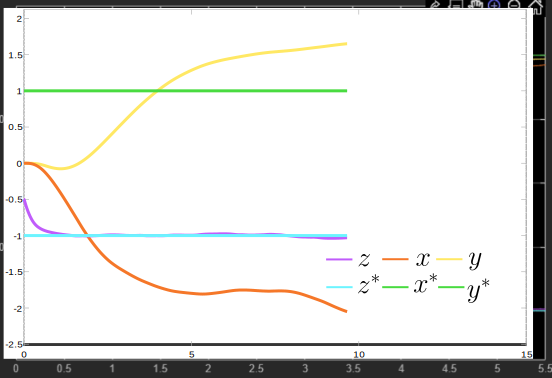
\includegraphics[width=1\linewidth]{wiatr/duzy}
	\caption{Przebiegi dla dużego wiatru}
	\label{fig:duzy}
\end{figure}

\section*{Podsumowanie projektu}
Zaprojektowany algorytm, który umożliwia zadawanie śmigłowcowi punktów drogi,
otwiera możliwości implementacji i dalszego rozwoju środowiska. Przykładowo,
można zastosować algorytmy planowania trasy do generowania macierzy zadanych
punktów. W trakcie realizacji projektu można także zwrócić uwagę na niezbędne czujniki,
które są kluczowe w takich aplikacjach. Aby dron mógł poprawnie realizować zadane 
algorytmy, konieczne są m.in. czujniki GPS, kamery oraz IMU, często w konfiguracjach
redundantnych i komplementarnych. Fundamentem sterowania systemami
autonomicznymi jest dostęp do pokładowych przyrządów pomiarowych, które zapewniają 
dokładność wymaganą dla danego zastosowania.

Moduł automatycznego lądowania wymaga praktycznej weryfikacji, gdyż symulowanie
zjawisk, takich jak turbulencje spowodowane przez reakcję podłoża, jest trudne.
Ze względu na ten problem konieczne jest dostrojenie algorytmu lądowania do warunków
środowiska, szczególnie w zakresie odpowiedniego sterowania ciągiem silników na różnych
wysokościach i fazach lądowania, by precyzyjnie określić moment ich wyłączenia.

Zakłócenia tj. wiatr mają wpływ na pracę układu, jednak to zależy jaka jest siła zakłóceń. W wielką burzę nic nie będzie latać. Ostatecznym wnioskiem jest to, że układ działa poprawnie. 
\clearpage
\end{document}